\section{Materials}\label{sec:Materials}

\begin{figure*}[h]
    \centering
    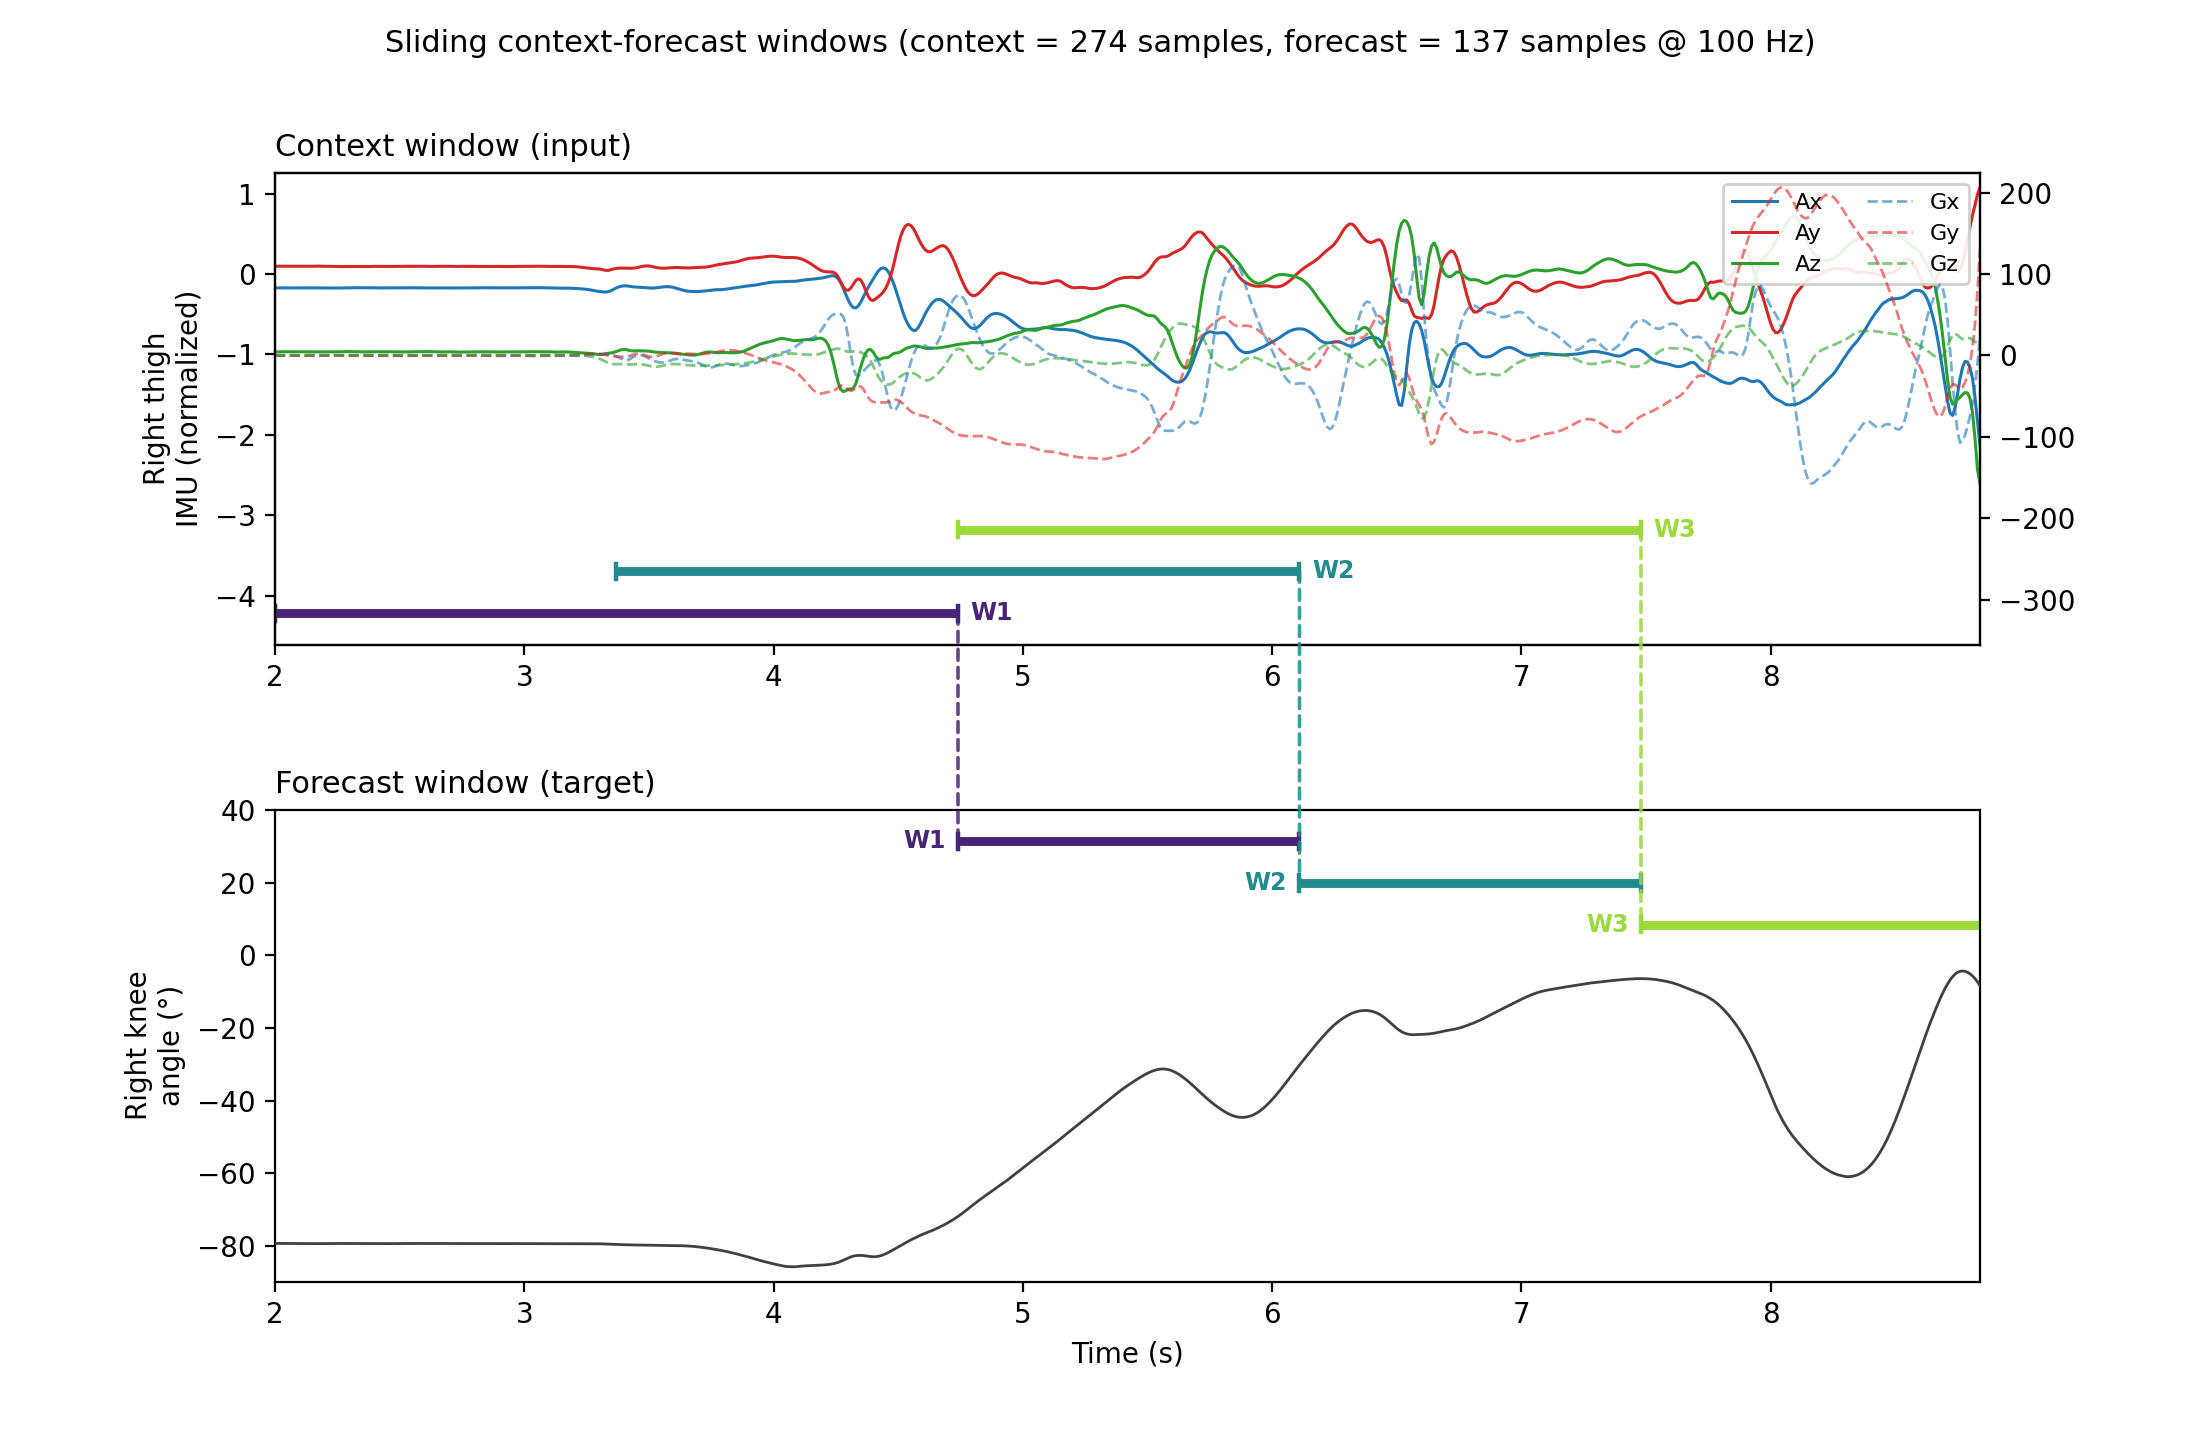
\includegraphics[width=\textwidth]{img/windowing_diagram.png}
    \caption{Sliding context-forecast windowing scheme applied to a representative
    trial. The top panel shows the right thigh IMU signals ($A_x, A_y, A_z$ solid,
    $G_x, G_y, G_z$ dashed)
    bottom panel shows the corresponding right knee goniometer signal with the matching forecast windows.}
    \label{fig:windowing_diagram}
\end{figure*}

\subsection{Dataset}
This study uses the ENcyclopedia of Able-bodied Bilateral Lower Limb Locomotor Signals 
(ENABL3S) dataset \citep{Hu2018}, introduced by Hu, Rouse, and Hargrove (2018) and 
publicly available on Figshare. It was designed as a benchmark for lower-limb 
neuromechanical signals recorded with wearable sensors during unassisted locomotion.

Ten healthy, able-bodied subjects (7 male, 3 female; age $25.5 \pm 2$ years; height 
$174 \pm 12$ cm; weight $70 \pm 14$ kg) participated. Subjects were instrumented 
bilaterally with surface EMG, electrogoniometers at the knee and ankle, and 6-DOF IMUs 
placed on the thigh, shank, and waist. Goniometer and IMU signals were sampled at 500 Hz. 
Each subject completed approximately 25 repetitions of a locomotion circuit encompassing 
sitting, standing, level-ground walking, ramp ascent/descent ($10°$ slope), and stair 
ascent/descent (four steps, 7.75 in. rise) at a self-selected comfortable speed.

This study uses exclusively the bilateral thigh-mounted IMUs as input, providing six 
channels of inertial data per leg: three axes of linear acceleration ($A_x, A_y, A_z$, 
in $g$) and three axes of angular velocity ($G_x, G_y, G_z$, in $°/s$), sampled at 
500 Hz. The prediction target is the continuously recorded right knee goniometer angle 
(in degrees). This single-sensor configuration is motivated by its practical relevance to 
prosthetic and exoskeleton control, where a thigh-mounted IMU on the proximal segment 
represents a minimally invasive setup. Left and right legs are treated independently, 
reflecting their distinct biomechanical profiles and effectively doubling the number of 
available training samples.

\subsection{Preprocessing}
Due to missing gait cycles, the Standing and Sitting activity classes were excluded from 
the analysis. The remaining signals were downsampled from 500 Hz to 100 Hz, preserving 
all frequency content relevant to human gait, which is predominantly below 20 Hz.

The downsampled signals were segmented into fixed-length windows. Each sample consists 
of a context window of 274 time steps representing the historical input sequence, and a 
forecast window of 137 time steps representing the prediction target. These values are based on the average gait of the dataset (137). Ensuring the model predicting a full gait cycle based on the past two cycles.

Prior to windowing, a height-based normalization is applied to reduce inter-subject
variability arising from differences in body size. Each subject's raw IMU signals are
scaled using their recorded height $h_i$ relative to a reference height $h_\text{ref}$,
defined as the cohort mean ($h_\text{ref} \approx 173.8$\,cm).
Biomechanical scaling theory predicts that peak linear accelerations during locomotion
are inversely proportional to leg length, while angular velocities follow a square-root
relationship with limb length through pendulum-like swing dynamics \cite{PLACEHOLDER}.
% TODO: verify cite key
Accordingly, the three accelerometer channels are multiplied by

\begin{equation}
    s_a = \frac{h_\text{ref}}{h_i},
    \label{eq:accel_scale}
\end{equation}

\noindent and the three gyroscope channels are multiplied by

\begin{equation}
    s_g = \sqrt{\frac{h_i}{h_\text{ref}}}.
    \label{eq:gyro_scale}
\end{equation}

\noindent This projection maps every subject's signals onto a common reference body,
reducing the component of inter-subject IMU variation attributable to morphology rather
than gait kinematics.

\noindent While the height projection compensates for the morphological component
of inter-subject variability, residual differences in signal amplitude persist,
arising from sensor placement, soft-tissue artefacts, and individual gait dynamics.
To remove this remaining scale variation, a second normalisation stage is applied
per subject. For each subject $i$ and each input channel $c$, the per-feature
minimum $m_i^c$ and maximum $M_i^c$ are computed across all of that subject's
windows, and every value is rescaled to the range $[-1, 1]$:

\begin{equation}
    \tilde{x}_i^c = 2 \cdot \frac{x_i^c - m_i^c}{M_i^c - m_i^c} - 1.
    \label{eq:per_subject_minmax}
\end{equation}

\noindent Crucially, the statistics $m_i^c$ and $M_i^c$ are derived from each
subject in isolation, including the held-out test subject under the LOSO protocol
described below. Because no subject is ever scaled using another subject's
statistics, this per-subject calibration introduces no information leakage between
the training and test folds, while mapping all subjects onto a common dynamic range.
This reflects the realistic deployment assumption that a short, unlabelled
calibration recording --- sufficient to estimate per-channel signal ranges --- can
be obtained from a new user before inference.

To evaluate generalisation to unseen individuals, a Leave-One-Subject-Out (LOSO) 
cross-validation scheme was adopted. In each fold, one subject is held out entirely as 
the test set, while the remaining subjects are split into training (90\%) and validation 
(10\%) sets at the subject level to prevent data leakage --- a critical consideration 
given the high within-subject temporal autocorrelation of IMU signals. This scheme 
reflects the real-world deployment scenario in which the model must generalise to a new 
user without subject-specific calibration data.